\documentclass[11pt]{article}

\usepackage[margin=1in]{geometry}
\usepackage{amsmath,amssymb}
\usepackage{paralist}
\usepackage{algorithm}
\usepackage{algpseudocode}
\usepackage{graphicx}
\usepackage{booktabs}


\newcommand{\N}{\mathbb{N}}
\newcommand{\Z}{\mathbb{Z}}

\begin{document}

\title{COMP 418/518: Homework 2 \\[1ex] \large [Weight of homework: 25\% of the final grade]}
\author{Dev Sanghvi (ds221), Ansh Dabral (ad258)}
\date{Due on February 25, 2026 \\ \small (released on February 6, 2026)}

\maketitle

\paragraph{Instructions:}

For this homework, you should work in groups of 3--4 people (i.e., the groups that have been declared and accepted).
%
Only one member of the group should submit on Gradescope.
%
All group members must be included in the submission on the Gradescope system (otherwise no credit will be given).
%
Also specify in your submission file all the members of your group (name and NetID) using the \texttt{\textbackslash authors} macro.
%
The submission must be typed in LaTeX using the provided template.
%
The use of AI systems (including, but not limited to, ChatGPT, Gemini, Copilot, and Claude) is entirely prohibited.
%
No discussion or collaboration is allowed outside of the group.
%
Late submissions are not accepted.

\begin{center}
You should provide \emph{pseudocode} for all the algorithms that you describe.
\end{center}

\paragraph{Note:}

We will request that you upload the LaTeX source for your submission. More information regarding how to make the source submission will be made available in a few days.

\paragraph{Grading:}

The homework will be graded based on correctness, completeness, and the quality of the provided solutions.

\newpage
\section*{Problem 1 [20 points]}

Many IoT applications involve the processing of signals that are generated by sensors. Processing these signals often involves \emph{filtering}, a signal processing technique used to remove noise from the signal. The moving (sliding) average that we have seen in class is an example of an \emph{FIR (Finite Impulse Response)} filter that removes high-frequency noise.

You are asked to design a streaming algorithm for another FIR filter, which is a sliding-window computation. The size of the window is $W$. Assume that the input stream consists of real numbers. At every step (after the first $W$ stream elements have been received), the filter should output the quantity
\[
  x_1 + 2 x_2 + 3 x_3 + \cdots + W x_W,
\]
where $x_1, \ldots, x_W$ are the last $W$ elements of the stream (i.e., the current window with $x_W$ being the most recent element).

Describe the most space- and time-efficient streaming algorithm that you can think of. Explain why your algorithm is correct. Give a precise description of the resources (space and time per item) that your algorithm uses.

\subsection*{Solution}

\textbf{Algorithm Description:}\\
We will maintain a circular buffer to store the elements of the current window.\\ \\
Variables being maintained:
\begin{enumerate}
    \item S: The simple sum of the elements in the current window.
    \item O: The weighted sum of the elements in the current window (your target output).
\end{enumerate}

\begin{algorithm}[H]
\caption{Streaming FIR Filter ($W$-size window)}
\begin{algorithmic}[1]
\State \textbf{Initialization:}
\State Read the first $W$ elements into an array \textit{buffer} of size $W$.
\State $S \gets \sum_{i=1}^{W} \textit{buffer}[i-1]$
\State $O \gets \sum_{i=1}^{W} i \cdot \textit{buffer}[i-1]$
\State $\textit{idx} \gets 0$ \Comment{Pointer to the oldest element}
\State \textbf{Output} $O$
\State \textbf{Streaming Update} (for each new element $x_{\text{new}}$):
\State $x_{\text{old}} \gets \textit{buffer}[\textit{idx}]$
\State $O \gets O - S + W \cdot x_{\text{new}}$
\State $S \gets S - x_{\text{old}} + x_{\text{new}}$
\State $\textit{buffer}[\textit{idx}] \gets x_{\text{new}}$ \Comment{Overwrite oldest element}
\State $\textit{idx} \gets (\textit{idx} + 1) \bmod W$ \Comment{Update index circularly}
\State \textbf{Output} $O$
\end{algorithmic}
\end{algorithm}

\newpage

\textbf{Proof of Correctness:}
To prove the algorithm is correct, we must show that our update rule produces the correct new weighted sum algebraically.\\
Let the previous window consist of elements $x_1, x_2, \dots, x_W$, where $x_1$ is the oldest and $x_W$ is the most recent. Our running variables represent the following:
\begin{align*}
    S &= x_1 + x_2 + x_3 + \dots + x_W \\
    O &= 1x_1 + 2x_2 + 3x_3 + \dots + Wx_W
\end{align*}
When a new element $x_{\text{new}}$ arrives, the new window becomes $x_2, x_3, \dots, x_W, x_{\text{new}}$. The correct new weighted sum $O_{\text{new}}$ that the filter should output is:
\[
O_{\text{new}} = 1x_2 + 2x_3 + \dots + (W-1)x_W + Wx_{\text{new}}
\]
Let's evaluate the algebraic expression used in our streaming algorithm, $O - S$:
\[
O - S = (1x_1 + 2x_2 + 3x_3 + \dots + Wx_W) - (x_1 + x_2 + x_3 + \dots + x_W)
\]
Subtracting term by term, the $x_1$ cancels out completely, and the coefficients for the rest of the terms decrease by exactly 1:
\[
O - S = 1x_2 + 2x_3 + \dots + (W-1)x_W
\]
Notice that $O - S$ neatly handles the shifted weights for all the surviving elements from the previous window. To get the final $O_{\text{new}}$, we just need to add the new element multiplied by its maximum weight, $W$:
\[
(O - S) + Wx_{\text{new}} = 1x_2 + 2x_3 + \dots + (W-1)x_W + Wx_{\text{new}}
\]
This precisely matches $O_{\text{new}}$. The simple sum is also updated correctly:
\[
S_{\text{new}} = S - x_1 + x_{\text{new}} = x_2 + x_3 + \dots + x_W + x_{\text{new}}
\]
Because the simple sum $S$ is always correctly maintained, the weighted sum $O$ will continue to be correctly computed in all subsequent streaming steps.\\ \\
\textbf{Resources: }\\
\textbf{Time per item:} $O(1)$. After the initial window is filled, processing every subsequent item from the stream requires a strictly fixed number of operations: two additions/subtractions, one multiplication, one array read, one array write, and one modulo operation. This computational cost is entirely independent of the window size $W$, making it optimally efficient for real-time IoT streaming.\\
\textbf{Space:} $O(W)$. We must maintain a circular buffer of size $W$ to store the past elements so we can accurately retrieve and subtract the oldest element ($x_{\text{old}}$) from our running sum. We also use a few scalar variables ($S$, $O$, $\textit{idx}$), which take $\mathcal{O}(1)$ space. The overall space complexity is dominated by the buffer, resulting in $\mathcal{O}(W)$ space. This is the absolute minimum space required; without storing the actual elements of the window, you cannot exactly identify and subtract the exiting element's contribution.\\

\newpage
\section*{Problem 2 [30 points]}

Suppose that the input stream is a sequence of measurements from a smart IoT sensor. The measurements are integers, i.e., elements of $\Z = \{ \ldots, -2, -1, 0, 1, 2, \ldots \}$. We use the notation $x[n]$, where $n \in \N$, for the input stream. We also call $x$ the \emph{input signal}. The value $x[n]$ is the sensor measurement at time instant $n$.

We want to perform a sliding-window computation, where $W \geq 2$ is the size of the window. The window at a time instant $n \in \N$ contains the measurements
\[
  x[\max(0, n - W + 1)], \ldots, x[n-1], x[n]
  \ .
\]
For example, if $W = 3$, then the window at time instant $n = 5$ contains the measurements $x[3], x[4], x[5]$.
%
We use the notation $y[n]$, where $n \in \N$, for the output stream we want to compute, i.e., the \emph{output signal}. The value $y[n]$ is the output at time instant $n$. Let $T_1, T_2 \in \Z$ be two \emph{threshold} values that satisfy $T_1 < T_2$. Define the output value
\[
  y[n] = \begin{cases}
    1, &\text{$x[i] \in [T_1,T_2)$ and $x[j] \in [T_2,\infty)$ for some $i, j \in \{\max(0,n-W+1),\ldots,n\}$ with $i < j$}
    \\
    0, &\text{otherwise}
  \end{cases}
\]
for every time instant $n \in \N$. In other words, $y[n] = 1$ iff the window (at time instant $n$) contains a measurement in the interval $[T_1, T_2) = \{ v \mid T_1 \leq v < T_2 \}$ followed by a measurement in the interval $[T_2, \infty) = \{ v \mid v \geq T_2 \}$.

Describe the most space- and time-efficient streaming algorithm that you can think of for this sliding-window computation. Explain why your algorithm is correct. Give a precise description of the resources (space and time per item) that your algorithm uses.

\subsection*{Solution}

\subsection*{Algorithm Description}

The problem asks us to output $y[n] = 1$ if the current window of size $W$ contains a measurement in $[T_1, T_2)$ followed by a measurement in $[T_2, \infty)$. \\
Instead of maintaining a buffer of the last $W$ measurements, we only need to keep track of the \textit{most recent} indices that satisfy these conditions. Let $(i, j)$ be a pair of indices such that $i < j$, $x[i] \in [T_1, T_2)$, and $x[j] \ge T_2$. We call this a ``valid pair''. For $y[n]$ to be $1$, there must exist a valid pair within the current window.\\ \\
We maintain two state variables:
\begin{enumerate}
    \item $\textit{idx}_{T1}$: The index of the most recently seen measurement in $[T_1, T_2)$.
    \item $\textit{idx}_{success}$: The index $i$ of the most recent valid pair $(i, j)$.
\end{enumerate}

\begin{algorithm}[H]
\caption{Streaming IoT Threshold Detection}
\begin{algorithmic}[1]
\State \textbf{Initialization:}
\State $\textit{idx}_{T1} \gets -1$ \Comment{Tracks the latest index $i$ where $x[i] \in [T_1, T_2)$}
\State $\textit{idx}_{success} \gets -1$ \Comment{Tracks the latest $i$ that forms a valid pair}
\State $n \gets 0$ \Comment{Current time instant}
\State \textbf{Streaming Update} (for each new measurement $x[n]$):
\If{$T_1 \le x[n] < T_2$}
    \State $\textit{idx}_{T1} \gets n$
\ElsIf{$x[n] \ge T_2$}
    \State $\textit{idx}_{success} \gets \textit{idx}_{T1}$
\EndIf
\If{$\textit{idx}_{success} \ge \max(0, n - W + 1)$}
    \State $y[n] \gets 1$
\Else
    \State $y[n] \gets 0$
\EndIf
\State \textbf{Output} $y[n]$
\State $n \gets n + 1$
\end{algorithmic}
\end{algorithm}

\subsection*{Correctness}

To prove correctness, we must show that $y[n]=1$ if and only if a valid pair $(i, j)$ exists within the window $[\max(0, n-W+1), n]$.\\
\textbf{1.} For a valid pair $(i, j)$ to be in the current window, we must have $\max(0, n-W+1) \le i < j \le n$. Notice that because $j > i$, if $i$ is inside the window bound ($i \ge n-W+1$), $j$ is guaranteed to be inside the window bound as well (since $j$ arrived at or before step $n$). Therefore, the survival of the pair in the sliding window depends \textit{entirely} on whether index $i$ has fallen out of the window.\\
\textbf{2.} Suppose there are multiple valid pairs in the stream. The pair that will survive the longest in the sliding window is the one with the maximum starting index $i$. \\
Our algorithm tracks the most recent $x[k] \in [T_1, T_2)$ using $\textit{idx}_{T1}$. Thus, $\textit{idx}_{T1}$ is always the largest possible starting index available.\\
Whenever a valid closing element $x[n] \ge T_2$ arrives, it forms a pair with the most recently seen starting element. We update $\textit{idx}_{success} \gets \textit{idx}_{T1}$. This locks in the largest known index $i$ that is part of a valid pair.\\
\textbf{3.} Finally, the algorithm outputs $1$ if $\textit{idx}_{success} \ge \max(0, n - W + 1)$. This correctly checks if the best possible starting index $i$ is still within the current bounds of the sliding window. If the best $i$ has expired (fallen out), then all older starting indices have also expired, meaning no valid pairs remain, and the algorithm correctly outputs $0$.

\subsection*{Resources}

\textbf{Time per item:} $\mathbf{\mathcal{O}(1)}$. Processing a new item requires at most two comparisons to check the thresholds, one assignment to update the state variables, one subtraction to calculate the window bound, and one comparison to determine $y[n]$. This is strictly constant time per measurement.\\
\textbf{Space:} $\mathbf{\mathcal{O}(1)}$. Unlike standard sliding window algorithms that require $\mathcal{O}(W)$ space to maintain a buffer, this algorithm does not need to remember the measurements themselves. We only store three scalar integers: $\textit{idx}_{T1}$, $\textit{idx}_{success}$, and $n$. Thus, the space complexity is optimally $\mathcal{O}(1)$ regardless of the window size $W$.\\

\section*{Problem 3 [15 points]}

Recall from the lectures the ``sliding max'' problem, that is, the streaming problem of calculating the maximum over a sliding window.

Give an algorithm for the sliding max problem with worst-case time per item $O(\log W)$, where $W$ is the size of the window. Explain why your algorithm is correct. What is the space and total time complexity of your algorithm?

\subsection*{Solution}

\subsection*{Algorithm Description}

While a deque-based approach provides $\mathcal{O}(1)$ amortized time, its worst-case time per item can be $\mathcal{O}(W)$. To strictly bound the worst-case time per item to $\mathcal{O}(\log W)$, we can use a \textbf{Balanced Binary Search Tree (BBST)} paired with a \textbf{circular buffer}.\\
The circular buffer keeps track of the chronological arrival of the items so we know exactly which item is expiring and needs to be removed. The BBST maintains the sorted order of the elements currently in the window, allowing us to query the maximum efficiently.\\ \\ 
We maintain the following structures:\\
\textit{Tree}: A BBST that stores the elements of the current window.\\
\textit{Buffer}: An array of size $W$ that acts as a circular queue.\\
$\textit{idx}$: A counter modulo $W$ to track the oldest element in the buffer.\\


\begin{algorithm}[H]
\caption{Sliding Max with $\mathcal{O}(\log W)$ worst-case time}
\begin{algorithmic}[1]
\State \textbf{Initialization:}
\State Initialize an empty BBST \textit{Tree}.
\State Initialize an array \textit{Buffer} of size $W$.
\State $\textit{idx} \gets 0$
\State $n \gets 0$ \Comment{Number of elements processed}
\State \textbf{Streaming Update} (for each new element $x[n]$):
\If{$n \ge W$}
    \State $x_{\text{old}} \gets \textit{Buffer}[\textit{idx}]$
    \State $\textit{Tree}.\text{removeOne}(x_{\text{old}})$ \Comment{Remove one instance of the expired element}
\EndIf
\State $\textit{Tree}.\text{insert}(x[n])$ \Comment{Insert the new element}
\State $\textit{Buffer}[\textit{idx}] \gets x[n]$ \Comment{Overwrite the oldest element in the buffer}
\State $\textit{idx} \gets (\textit{idx} + 1) \bmod W$ \Comment{Update circular pointer}
\If{$n \ge W - 1$}
    \State $\text{current\_max} \gets \textit{Tree}.\text{findMax}()$ \Comment{The largest element in the BBST}
    \State \textbf{Output} $\text{current\_max}$
\EndIf
\State $n \gets n + 1$
\end{algorithmic}
\end{algorithm}

\subsection*{Correctness}

The algorithm correctly computes the sliding window maximum because the data structures perfectly mirror the current state of the window at any time step $n$.\\
\textbf{Synchronization:} The circular buffer continuously holds exactly the last $W$ elements from the stream. When the window slides, the exact element that falls out of the $W$-sized window is identified by the buffer.\\
\textbf{Tree State:} By explicitly inserting the newest element $x[n]$ and strictly removing the exactly matched oldest element $x_{\text{old}}$ from the BBST, the tree is guaranteed to contain the exact same multiset of $W$ elements as the current sliding window.\\
\textbf{Max Query:} Because a BBST maintains its elements in sorted order, querying the maximum element (\textit{Tree.findMax()}) is guaranteed to return the correct maximum value among the current $W$ items.\\


\subsection*{Complexity Analysis}


\textbf{Worst-case time per item:} $\mathbf{\mathcal{O}(\log W)}$. 
For each incoming item, we perform at most one insertion and one deletion in the BBST. Because the BBST never contains more than $W$ elements, both \textit{insert} and \textit{remove} operations take strictly $\mathcal{O}(\log W)$ time in the worst case. Finding the maximum takes $\mathcal{O}(\log W)$ time (or $\mathcal{O}(1)$ if a pointer to the rightmost node is maintained). Array operations take $\mathcal{O}(1)$ time. Thus, the total worst-case time per item is bounded by $\mathcal{O}(\log W)$.\\ \\ 
\textbf{Space Complexity:} $\mathbf{\mathcal{O}(W)}$. 
The circular buffer stores exactly $W$ elements. The BBST also stores at most $W$ elements (with standard $\mathcal{O}(1)$ overhead per node for pointers and balance factors). Therefore, the overall space complexity is strictly $\mathcal{O}(W)$.\\ \\
\textbf{Total Time Complexity:} $\mathbf{\mathcal{O}(N \log W)}$. 
    If the total length of the input stream is $N$ items, and we process each item in $\mathcal{O}(\log W)$ worst-case time, the total time to process the entire stream is $\mathcal{O}(N \log W)$.


\newpage
\section*{Problem 4 [40 points]}

Suppose that the input items are drawn from the set $\{ 0, 1, \ldots, R-1 \}$, where $R$ is a (small) \emph{constant}.
\begin{enumerate}[\ (1)]
\item
Give a space-optimal (asymptotically) algorithm for the sliding max problem (the window size is $W$). Measure space (memory) in bits.
\item
Prove a space lower bound (for the problem) that matches the upper bound for your algorithm.
\end{enumerate}

\subsection*{Solution}

\subsubsection*{(1): Space-Optimal Algorithm}

Since the input values are restricted to a small constant set $\{0, 1, \dots, R-1\}$, we do not need to store the values themselves. Instead, we can simply keep track of the \textit{age} of the most recent occurrence of each possible value. If a value's age is less than $W$, it is currently inside the window.

We maintain an array $D$ of size $R$, where $D[v]$ stores the number of time steps since the value $v$ was last seen. If $v$ has not been seen in the last $W$ steps, we cap $D[v]$ at $W$.

\begin{algorithm}[H]
\caption{Space-Optimal Constant-Alphabet Sliding Max}
\begin{algorithmic}[1]
\State \textbf{Initialization:}
\State Initialize an array $D[0 \dots R-1]$ such that $D[v] = W$ for all $v$.
\State $n \gets 0$
\State \textbf{Streaming Update} (for each new element $x[n]$):
\For{$v \gets 0$ to $R-1$}
    \If{$D[v] < W$}
        \State $D[v] \gets D[v] + 1$ \Comment{Increment the age of all active values}
    \EndIf
\EndFor
\State $D[x[n]] \gets 0$ \Comment{The new element has an age of 0}
\If{$n \ge W - 1$}
    \State $\text{max\_val} \gets 0$
    \For{$v \gets R-1$ down to 0} \Comment{Check from largest possible value down}
        \If{$D[v] < W$}
            \State $\text{max\_val} \gets v$
            \State \textbf{break}
        \EndIf
    \EndFor
    \State \textbf{Output} $\text{max\_val}$
\EndIf
\State $n \gets n + 1$
\end{algorithmic}
\end{algorithm}

\subsubsection*{Space Complexity}
The algorithm maintains exactly $R$ integers. Because we cap the age at $W$, each integer $D[v] \in \{0, 1, \dots, W\}$. Storing a number up to $W$ requires $\lceil \log_2(W+1) \rceil$ bits. 
Therefore, the total space required is:
\[
S(W) = R \cdot \lceil \log_2(W+1) \rceil \text{ bits}
\]
Since $R$ is a constant, the asymptotic space complexity is strictly $\mathbf{\mathcal{O}(\log W)}$ \textbf{bits}.

\subsection*{(2): Space Lower Bound Proof}

To prove a matching lower bound of $\Omega(\log W)$ bits, we must show that any deterministic streaming algorithm requires at least this much memory to correctly answer sliding max queries. We will use a state-distinguishability argument.\\
Suppose the algorithm has processed a prefix of the stream. Its internal memory must encode enough information to answer all future queries correctly. Let us construct a family of adversarial window states of length $W$ that all require different memory states.\\
Consider strings of length $W$ over the alphabet $\{0, \dots, R-1\}$ that contain exactly one instance of each value $v \in \{1, 2, \dots, R-1\}$, and $0$ everywhere else. Let $p_v \in \{1, 2, \dots, W\}$ denote the index (position) of value $v$ inside this window. We restrict our family of strings to those where the non-zero values appear in strictly decreasing order from left to right. That is, their positions satisfy:
\[
1 \le p_{R-1} < p_{R-2} < \dots < p_1 \le W
\]

Suppose the algorithm has just processed one of these strings. Now, an adversary feeds a continuous stream of $0$s. 
\begin{itemize}
    \item Initially, the maximum is $R-1$.
    \item When exactly $W - p_{R-1}$ zeros have been appended, the value $R-1$ falls out of the sliding window. Because $p_{R-2} > p_{R-1}$, the value $R-2$ is still in the window. Thus, the output transitions exactly from $R-1$ to $R-2$.
    \item Generally, the output transitions from $k$ to $k-1$ exactly when $W - p_k$ zeros have been appended.
\end{itemize}

Because the exact number of zeros required to cause a drop in the maximum uniquely identifies the position $p_k$ for every $k \in \{1, \dots, R-1\}$, \textbf{any two strings with a different set of positions must produce a different sequence of future outputs.} Therefore, the algorithm must be in a strictly different internal memory state for every valid combination of positions.

How many such combinations exist? We are choosing $R-1$ distinct positions out of $W$ possible slots. The number of valid states is exactly:
\[
\binom{W}{R-1}
\]

By information theory, to uniquely represent at least $\binom{W}{R-1}$ different states, the algorithm requires $M$ bits of memory, where:
\[
M \ge \log_2 \binom{W}{R-1}
\]
Using the definition of the binomial coefficient:
\[
\log_2 \binom{W}{R-1} = \log_2 \left( \frac{W(W-1)\dots(W-R+2)}{(R-1)!} \right)
\]
For large $W$ and constant $R$, this is dominated by the $W^{R-1}$ term:
\[
M \ge (R-1) \log_2 W - \log_2((R-1)!)
\]
Because $R$ is a constant, $(R-1)$ is a constant factor and $\log_2((R-1)!)$ is a constant term. Therefore, the memory space required is:
\[
M = \mathbf{\Omega(\log W)} \text{ bits}
\]
This lower bound matches the $\mathcal{O}(\log W)$ bit upper bound of our algorithm, proving that the algorithm is asymptotically space-optimal.

\newpage
\section*{Problem 5 [20 points]}

An \textbf{\em IoT device A} generates \emph{messages} that are nested lists/sets of (arbitrarily large) natural numbers. We will define now the set $D$, which should be thought of as an abstract mathematical representation of such messages. Formally, $D$ is the smallest set that satisfies the following properties (which are implicitly universally quantified):
\begin{enumerate}
\item{}
[Number] If $n \in \N$ then $n \in D$ (``every natural number is a message'').
\item{}
[List] If $x_1, x_2, \ldots, x_n \in D$ then $[x_1, x_2, \ldots, x_n] \in D$.
\item{}
[Set] If $x_1, x_2, \ldots, x_n \in D$ then $\{ x_1, x_2, \ldots, x_n \} \in D$.
\end{enumerate}
Empty lists $[\,]$ and empty sets $\{ \}$ are messages. For example, $[ 4, \{ 2, 3 \}, [1, 2, \{ \} ], [6, [\,]], 7 ]$ is a message.
%
The messages are transmitted in serialized form, where numbers are represented as sequences of decimal digits. A \emph{serialized message} is a sequence over the following alphabet $\Sigma$ of symbols:
\begin{center}
\tt
0 1 2 3 4 5 6 7 8 9 [ ] \{ \} ,
\end{center}
It is also allowed to have (any number of) space symbols separating numbers, commas, brackets, and braces. For example, this is a serialized message (observe the presence of space symbols):
\begin{center}
\tt
[4, \{2, 3\}, [1, 2, \{\}], [6, [\,]], 7]
\end{center}
The \textbf{\em IoT device B} receives a stream over $\Sigma$ (\textbf{\em message stream}), which should be a sequence of serialized messages that are separated by (any number of) space symbols. For example,
\begin{center}
\tt
[ ] 100 \{1\} [2, 3] [4, \{7,8\}, 5] \{ \}
\end{center}
is a stream that consists of 6 complete serialized messages.

Describe a streaming algorithm for Device B that processes an input message stream. As soon as the algorithm sees a complete (serialized) message, it should output the total number of messages processed so far. This means that the algorithm should not produce output at every step. As soon as the algorithm notices that a message is \emph{malformed} (e.g., \texttt{[1, 2\}} or \texttt{[1, [2, 3]]]} or \texttt{[1, 2,]}), it should start emitting the error value $-1$ at every step.

Explain why your algorithm is correct. Give a precise description of the resources (space and time per item) that your algorithm uses.

\subsection*{Solution}

\subsubsection*{Algorithm Overview}

We use a \textbf{finite-state automaton} combined with a \textbf{stack} $S$ to track bracket/brace nesting. The automaton has five normal states plus an error state:
\begin{itemize}
\item \texttt{TOP}: Between top-level messages. Expecting the start of a new message or a space.
\item \texttt{NUM}: Reading digits of a number.
\item \texttt{OPEN}: Just opened a bracket/brace. Expecting an element or a matching close.
\item \texttt{SEP}: Just saw a comma. Expecting the next element.
\item \texttt{ELEM}: Just finished an element inside a list/set. Expecting a comma or a matching close.
\item \texttt{ERR}: Malformed input detected. Emit $-1$ at every subsequent step.
\end{itemize}
We also maintain a counter $C$ (number of complete messages).


\subsubsection*{Pseudocode}

\begin{algorithm}[H]
\caption{Streaming Message Parser (Part 1)}
\begin{algorithmic}[1]
\State \textbf{Initialization:}
\State $\text{state} \gets \texttt{TOP}$ \Comment{Current parser state}
\State $S \gets \text{empty stack}$ \Comment{Tracks bracket/brace nesting}
\State $C \gets 0$ \Comment{Number of complete messages}

\State \textbf{Streaming Update} (for each new symbol $\sigma \in \Sigma$):
\If{$\text{state} = \texttt{ERR}$}
    \State \textbf{Output} $-1$
    \State \Return
\EndIf

\State $\textit{emit\_C} \gets \text{false}$ \Comment{Flag to buffer output until step end}

\If{$\text{state} = \texttt{NUM} \land S\text{ is empty} \land \sigma \text{ is not a digit}$}
    \State $C \gets C + 1$
    \State $\textit{emit\_C} \gets \text{true}$
    \State $\text{state} \gets \texttt{TOP}$
\EndIf

\If{$\sigma$ is a space}
    \If{$\text{state} = \texttt{NUM} \land S\text{ is non-empty}$}
        \State $\text{state} \gets \texttt{ELEM}$
    \EndIf
\EndIf

\If{$\sigma$ is a digit}
    \If{$\text{state} \in \{\texttt{TOP}, \texttt{OPEN}, \texttt{SEP}\}$}
        \State $\text{state} \gets \texttt{NUM}$
    \ElsIf{$\text{state} = \texttt{ELEM}$}
        \State $\text{state} \gets \texttt{ERR}$
    \EndIf
\EndIf

\If{$\sigma \in \{\text{[}, \text{\{}\}$ (open bracket/brace)}
    \If{$\text{state} \in \{\texttt{TOP}, \texttt{OPEN}, \texttt{SEP}\}$}
        \State $\text{push } \sigma \text{ onto } S$
        \State $\text{state} \gets \texttt{OPEN}$
    \Else
        \State $\text{state} \gets \texttt{ERR}$
    \EndIf
\EndIf

\algstore{myalg}
\end{algorithmic}
\end{algorithm}

\addtocounter{algorithm}{-1}
\begin{algorithm}[H]
\caption{Streaming Message Parser (Part 2)}
\begin{algorithmic}[1]
    \algrestore{myalg}

\If{$\sigma \in \{\text{]}, \text{\}}\}$ (close bracket/brace)}
    \If{$\text{state} = \texttt{SEP}$}
        \State $\text{state} \gets \texttt{ERR}$
    \ElsIf{$\text{state} \in \{\texttt{NUM}, \texttt{OPEN}, \texttt{ELEM}\} \land S\text{ is non-empty}$}
        \State $o \gets S.\text{top}()$
        \If{$(o = \text{[} \land \sigma = \text{]}) \lor (o = \text{\{} \land \sigma = \text{\}})$}
            \State $\text{pop } S$
            \If{$S\text{ is empty}$}
                \State $C \gets C + 1$
                \State $\text{state} \gets \texttt{TOP}$
                \State $\textit{emit\_C} \gets \text{true}$
            \Else
                \State $\text{state} \gets \texttt{ELEM}$
            \EndIf
        \Else
            \State $\text{state} \gets \texttt{ERR}$
        \EndIf
    \Else
        \State $\text{state} \gets \texttt{ERR}$
    \EndIf
\EndIf

\If{$\sigma = \text{,}$}
    \If{$\text{state} \in \{\texttt{NUM}, \texttt{ELEM}\} \land S\text{ is non-empty}$}
        \State $\text{state} \gets \texttt{SEP}$
    \Else
        \State $\text{state} \gets \texttt{ERR}$
    \EndIf
\EndIf

\If{$\text{state} = \texttt{ERR}$}
    \State \textbf{Output} $-1$ \Comment{Prioritize error reporting}
\ElsIf{$\textit{emit\_C}$}
    \State \textbf{Output} $C$
\EndIf
\end{algorithmic}
\end{algorithm}

\subsubsection*{Correctness}

The automaton enforces the grammar of valid messages:
\begin{itemize}
\item A message is either a number (sequence of digits), a list \texttt{[$\ldots$]}, or a set \texttt{\{$\ldots$\}}.
\item List/set elements are separated by commas. Empty lists \texttt{[\,]} and sets \texttt{\{\,\}} are allowed (via the \texttt{OPEN} $\to$ close transition).
\item The stack $S$ ensures correct nesting and matching of brackets/braces.
\item Transitions to \texttt{ERR} capture all malformed cases: mismatched brackets (\texttt{[1,2\}}), extra closing brackets (\texttt{[1,[2,3]]]}), trailing commas (\texttt{[1,2,]}), missing commas, commas at top level, and double commas.
\item Upon detecting a malformed condition, the algorithm transitions to \texttt{ERR} and \textbf{immediately} outputs $-1$ on the exact same step, as well as at every subsequent step.
\item Top-level numbers do not require a trailing space to be considered complete; the algorithm detects the end of a top-level number natively upon encountering any non-digit character (like `[' or `\{') or via the absence of items on the stack.
\end{itemize}

\textbf{Example trace.} For the stream ``\texttt{[ ] 100 \{1\}}'', the algorithm transitions: \texttt{TOP} $\xrightarrow{[}$ \texttt{OPEN} $\xrightarrow{\text{\textvisiblespace}}$ \texttt{OPEN} $\xrightarrow{]}$ \texttt{TOP} (output $C\!=\!1$) $\xrightarrow{\text{\textvisiblespace}}$ \texttt{TOP} $\xrightarrow{1}$ \texttt{NUM} $\xrightarrow{0}$ \texttt{NUM} $\xrightarrow{0}$ \texttt{NUM} $\xrightarrow{\text{\textvisiblespace}}$ \texttt{TOP} (output $C\!=\!2$) $\xrightarrow{\{}$ \texttt{OPEN} $\xrightarrow{1}$ \texttt{NUM} $\xrightarrow{\}}$ \texttt{TOP} (output $C\!=\!3$).

\subsubsection*{Resource Analysis}

\begin{itemize}
\item \textbf{Time per item:} $O(1)$. Each symbol requires a constant number of operations (check state, possibly push/pop the stack, update counter).
\item \textbf{Space:} $O(d_{\max} + \log n)$ bits, where $d_{\max}$ is the maximum nesting depth and $n$ is the stream length. The stack uses $d_{\max}$ bits (1 bit per level, distinguishing \texttt{[} from \texttt{\{}). The counter $C$ uses $O(\log n)$ bits. The automaton state uses $O(1)$ bits (one of 6 states $= 3$ bits). In the worst case, $d_{\max} = O(n)$ (e.g., \texttt{[[[...]]]}), so the space is $O(n)$ bits.
\end{itemize}
\newpage
\section*{Problem 6 [125 points]}

Implement the approximation algorithm for counting 1's over a sliding window using the provided code files. Include the benchmarking results and any other relevant information below.
\begin{itemize}[$-$]
\item
Zip up the entire folder with your solution (only the source code!) and submit it on Gradescope.
\item
Your implementation should only call malloc \textbf{\em once} (during the initialization of the state). After this call of malloc during initialization, there should be no other dynamic memory allocation. The purpose of this restriction is to be faithful to an embedded IoT device that has a small amount of memory and offers no dynamic memory allocation.
\item
All the data structures used by your algorithm should be implemented from scratch.
\end{itemize}

\subsection*{Solution}

\subsubsection*{Algorithm Overview}

We implement the DGIM (Datar--Gionis--Indyk--Motwani) approximation algorithm for counting 1's over a sliding window of size $W$. The algorithm maintains a collection of \emph{buckets}, where each bucket stores:
\begin{itemize}
\item A \textbf{timestamp} (the time of the most recent 1 it represents), and
\item A \textbf{power} $p$ (the bucket represents $2^p$ ones).
\end{itemize}

\noindent
Setting the parameter $k$ determines the accuracy: we allow at most $r + 1 = k + 1$ buckets per power level.

\subsubsection*{Data Structure}

We use \textbf{per-power-level ring buffers} (circular queues), each storing only timestamps for buckets of that power. Specifically:
\begin{itemize}
\item For each power level $p \in \{0, 1, \ldots, \lfloor \log_2 W \rfloor + 2\}$, we maintain a separate ring buffer of capacity $r + 2$.
\item All ring buffers are allocated from a \textbf{single contiguous block} via one call to \texttt{malloc}. The total memory is $(r + 2) \times (\text{number of power levels}) \times \text{sizeof}(\texttt{uint32\_t})$ bytes.
\item We also maintain a running \texttt{total\_sum} of all bucket sizes and a \texttt{highest\_power} tracker.
\end{itemize}

\noindent
This design achieves $O(1)$ amortized time per merge (just pop from one ring and push to another), and avoids any additional dynamic memory allocation after initialization.

\subsubsection*{Processing Each Item}

On each incoming bit:
\begin{enumerate}
\item \textbf{Expire}: Remove the oldest bucket (at the tail of the highest occupied power level) if its timestamp is outside the window.
\item \textbf{Insert}: If the bit is 1, push a new entry (timestamp, power 0) onto ring 0.
\item \textbf{Merge cascade}: Starting from power $p = 0$, if the ring for power $p$ has $r + 2$ entries, pop the two oldest, and push one merged entry (with the more recent of the two timestamps) onto the ring for power $p + 1$. Repeat for $p + 1$ if needed.
\item \textbf{Query}: Return $\texttt{total\_sum} - 2^{p_{\max}} + 1$, where $p_{\max}$ is the power of the oldest bucket.
\end{enumerate}

\subsubsection*{Estimate and Error Analysis}

The algorithm's estimate for the number of 1's is:
\[
  \hat{C} = \texttt{total\_sum} - 2^{p_{\text{oldest}}} + 1
\]
where $p_{\text{oldest}}$ is the power (size $2^{p_{\text{oldest}}}$) of the oldest (highest-power) bucket currently in the window.

\textbf{No overestimation:} The oldest bucket has not expired, meaning its timestamp (which corresponds to the most recent 1 it represents) is strictly inside the window. Therefore, at least 1 of its $2^{p_{\text{oldest}}}$ constituent 1's is guaranteed to be inside the window. Thus, the true count $C$ must be at least:
\[
  C \ge \texttt{total\_sum} - 2^{p_{\text{oldest}}} + 1 = \hat{C}
\]

\textbf{Rigorous Error Bound Proof:} 
The absolute error is bounded by the unknown remaining 1's tightly packed in the oldest bucket, which is at most $2^{p_{\text{oldest}}} - 1$. To bound the relative error $\epsilon = \frac{C - \hat{C}}{C}$, we must mathematically prove a lower bound on the true count $C$. 

By the construction of the DGIM merging rules, we only merge two buckets of size $2^{p-1}$ into a bucket of size $2^p$ when we encounter a total of $r + 2$ buckets of size $2^{p-1}$. After this merge, exactly $r$ buckets of size $2^{p-1}$ remain. Because we set $r = k$, this implies that the existence of \textbf{any} bucket of size $2^p$ strictly guarantees the existence of \textit{at least} $k$ buckets of size $2^{p-1}$, $k$ buckets of size $2^{p-2}$, and so on down to $k$ buckets of size $2^0$.

Therefore, if the oldest bucket has power $p_{\text{oldest}} = p$, the \texttt{total\_sum} of all buckets currently maintained by the algorithm is bounded below by the oldest bucket itself plus the guaranteed $k$ buckets at every smaller power level:
\begin{align*}
  \texttt{total\_sum} &\ge 2^p + \sum_{i=0}^{p-1} k \cdot 2^i \\
  &= 2^p + k(2^p - 1)
\end{align*}
Since the true count $C \ge \hat{C} = \texttt{total\_sum} - 2^p + 1$, we substitute our lower bound for \texttt{total\_sum}:
\[
  C \ge \left[ 2^p + k(2^p - 1) \right] - 2^p + 1 = k(2^p - 1) + 1
\]
The maximum possible absolute error is $2^p - 1$. Thus, the maximum relative error is strictly bounded by:
\[
  \text{Relative Error} = \frac{\text{error}}{C} \le \frac{2^p - 1}{k(2^p - 1) + 1} < \frac{2^p - 1}{k(2^p - 1)} = \frac{1}{k}
\]
By choosing $k \ge 1/\epsilon$, the relative error is guaranteed to be strictly less than $\epsilon$, satisfying the DGIM approximation guarantee. \hfill $\square$

\subsubsection*{Complexity}

\begin{itemize}
\item \textbf{Space}: $O(k \cdot \log W)$ timestamps $= O(k \log W)$ words. A single \texttt{malloc} call allocates all memory at initialization.
\item \textbf{Time per item}: $O(1)$ amortized. Each item causes at most one insertion and one expiry, both $O(1)$. Merges are amortized $O(1)$ since each bucket is merged at most $O(\log W)$ times over its lifetime.
\end{itemize}

\subsubsection*{Benchmarking Methodology \& Results}

\textbf{Experimental Setup:} The algorithms were compiled on an Apple Silicon processor using GCC with full optimizations via the command \texttt{gcc -O3 bench.c -o bench -lm}. We benchmarked over an adversarial stream of $50{,}000{,}000$ items \textit{(all 1's)}. This stream pattern represents the strict, pessimistic worst-case scenario for the DGIM algorithm, as every single bit insertion necessarily triggers a new bucket creation and maximizes the frequency of $O(\log W)$ merge cascades. The window sizes varied across $W \in \{10, \dots, 1{,}000{,}000\}$ and accuracy parameters $k \in \{10, 100, 1000\}$. Each configuration was run for 3 trials.

\textbf{Raw Benchmark Data:} The table below reports the memory footprint (bytes) and average throughput (Millions of items/sec) spanning all configurations. 

\begin{table}[ht!]
\centering
\begin{tabular}{l|r|rr|rr|rr}
\toprule
& \multicolumn{1}{c|}{\textbf{Exact}} & \multicolumn{2}{c|}{\textbf{Approx ($k=10$)}} & \multicolumn{2}{c|}{\textbf{Approx ($k=100$)}} & \multicolumn{2}{c}{\textbf{Approx ($k=1000$)}} \\
\textit{W} & Mem & Mem & TP & Mem & TP & Mem & TP \\
\midrule
10          & 10 B & 720 B & $\sim$200M     & 5,040 B & $\sim$176M     & 48,240 B & $\sim$196M \\
100         & 100 B & 1,080 B & $\sim$195M   & 7,560 B & $\sim$196M     & 72,360 B & $\sim$197M \\
1,000       & 1,000 B & 1,440 B & $\sim$197M   & 10,080 B & $\sim$176M    & 96,480 B & $\sim$202M \\
10,000      & 10,000 B & 1,920 B & $\sim$184M   & 13,440 B & $\sim$162M    & 128,640 B & $\sim$200M \\
100,000     & 100,000 B & 2,280 B & $\sim$205M   & 15,960 B & $\sim$182M    & 152,760 B & $\sim$192M \\
1,000,000   & 1,000,000 B & 2,640 B & $\sim$192M   & 18,480 B & $\sim$185M    & 176,880 B & $\sim$198M \\
\bottomrule
\end{tabular}
\caption{Raw benchmarking throughputs (Millions items/sec) and memory bounds (Bytes).}
\end{table}

\begin{figure}[ht!]
\centering
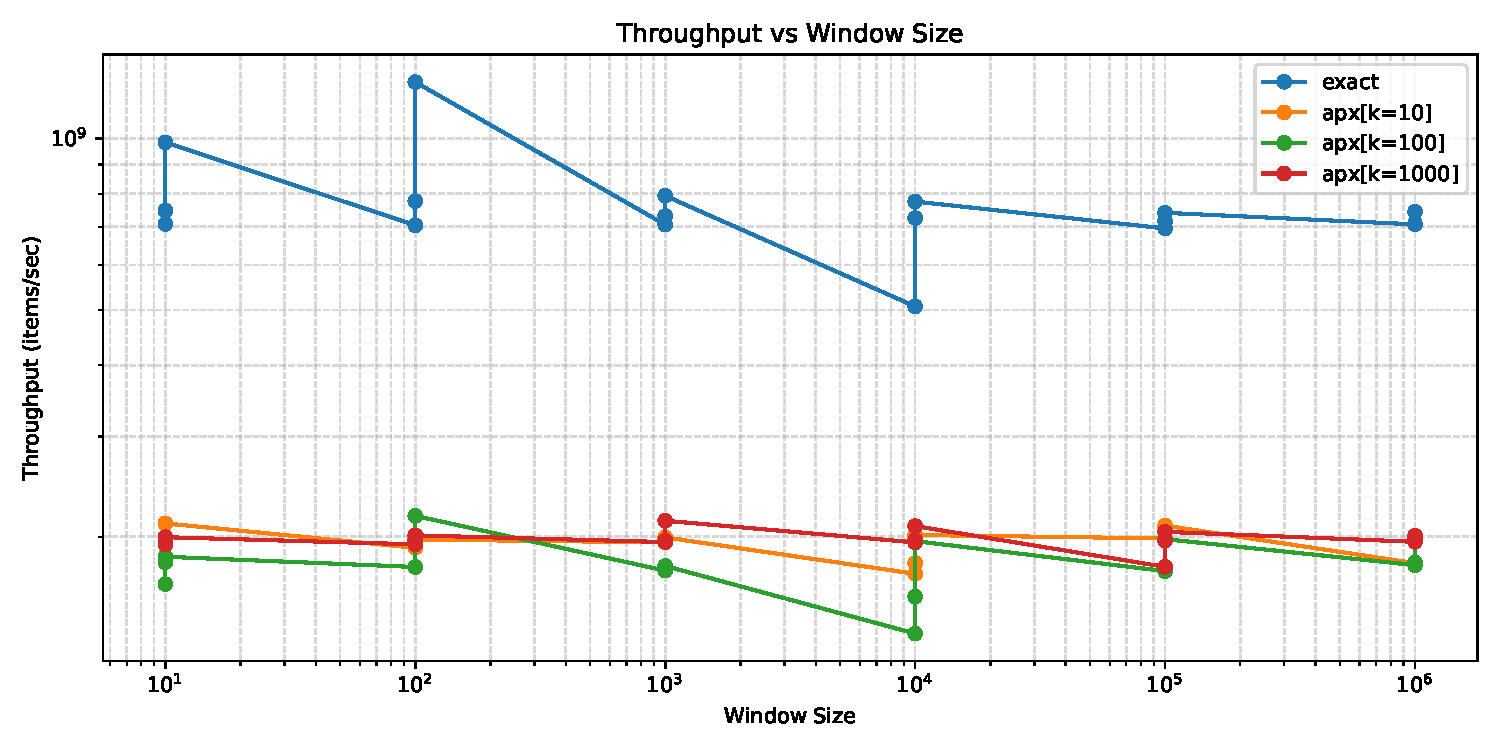
\includegraphics[width=0.95\textwidth]{throughput.pdf}
\caption{Throughput comparison (items/sec, log scale). The exact algorithm hits $\sim$760M items/sec on average regardless of $W$. Despite being stress-tested on its worst-case stream configuration mapping to continuous merge cascades, the approximate algorithm maintains a heavily robust throughput of $\sim$190M items/sec. Throughput remains relatively insensitive to $k$ and $W$.}
\end{figure}

\begin{figure}[ht!]
\centering
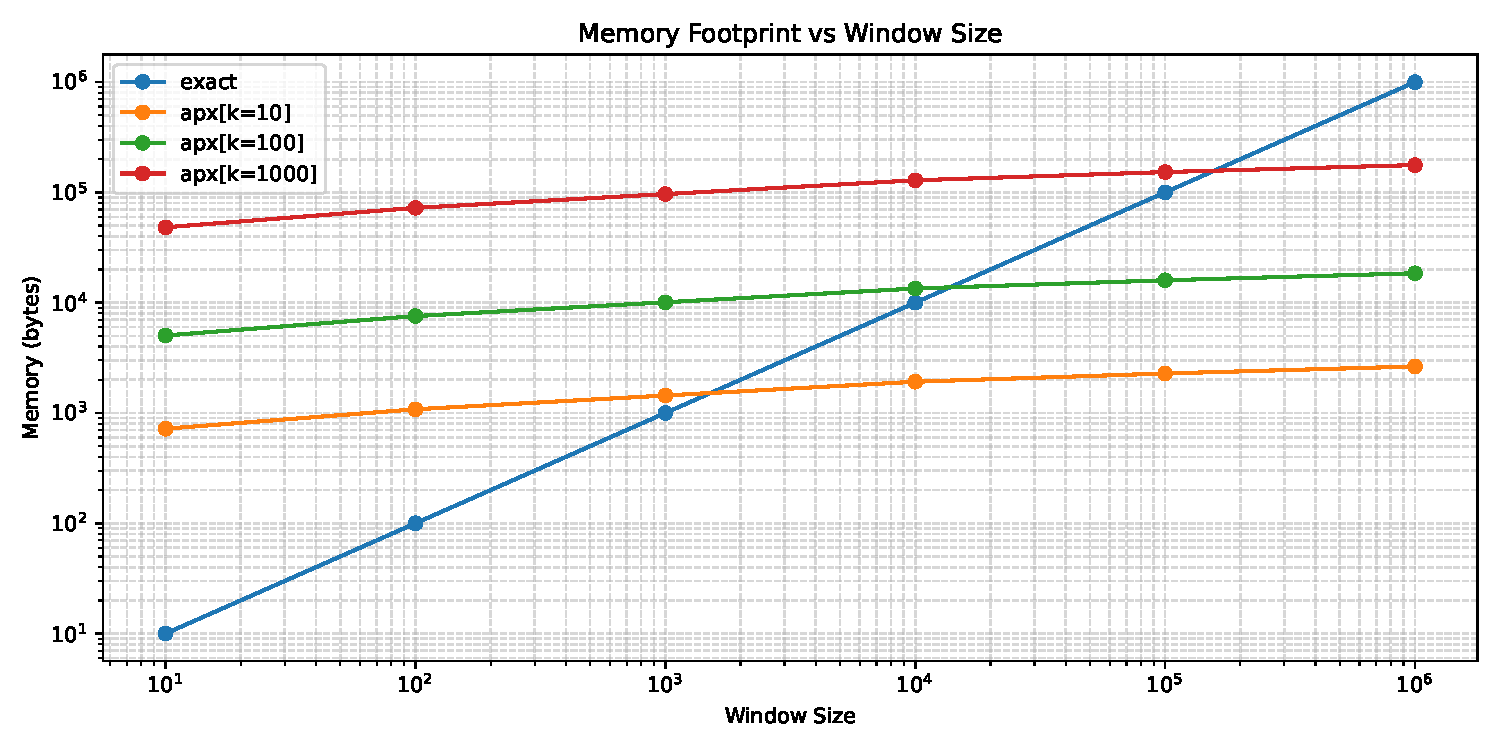
\includegraphics[width=0.95\textwidth]{memory_footprint.pdf}
\caption{Memory footprint comparison (bytes, log scale). The exact algorithm uses $W$ bytes ($\Theta(W)$). The approximate algorithm uses $O(k \log W)$ bytes --- for example, at $W = 1{,}000{,}000$ with $k = 10$, it uses only 2{,}640 bytes vs.\ 1{,}000{,}000 bytes for exact, a $\sim$378$\times$ reduction.}
\end{figure}

\bibliographystyle{plain}

\end{document}